\documentclass[12pt]{article}
\usepackage{amsmath}
\usepackage{graphicx}
\usepackage{hyperref}
\usepackage{listings}
\usepackage{color}
\usepackage{pythonhighlight}

\title{Operating System Course Report - First Half of the Semester}
\author{A class}
\date{\today}

\begin{document}

\maketitle
\newpage

\tableofcontents
\newpage

\section{Introduction}
This report summarizes the topics covered during the first half of the Operating System course. It includes theoretical concepts, practical implementations, and assignments. The course focuses on the fundamentals of operating systems, including system architecture, process management, CPU scheduling, and deadlock handling.

\section{Course Overview}
\subsection{Objectives}
The main objectives of this course are:
\begin{itemize}
    \item To understand the basic components and architecture of a computer system.
    \item To learn process management, scheduling, and inter-process communication.
    \item To explore file systems, input/output management, and virtualization.
    \item To study the prevention and handling of deadlocks in operating systems.
\end{itemize}

\subsection{Course Structure}
The course is divided into two halves. This report focuses on the first half, which covers:
\begin{itemize}
    \item Basic Concepts and Components of Computer Systems
    \item System Performance and Metrics
    \item System Architecture of Computer Systems
    \item Process Description and Control
    \item Scheduling Algorithms
    \item Process Creation and Termination
    \item Introduction to Threads
    \item File Systems
    \item Input and Output Management
    \item Deadlock Introduction and Prevention
    \item User Interface Management
    \item Virtualization in Operating Systems
\end{itemize}

\section{Topics Covered}

\subsection{Basic Concepts and Components of Computer Systems}
This section explains the fundamental components that make up a computer system, including the CPU, memory, storage, and input/output devices.

\subsection{System Performance and Metrics}
This section introduces various system performance metrics used to measure the efficiency of a computer system, including throughput, response time, and utilization.

\subsection{System Architecture of Computer Systems}
Describes the architecture of modern computer systems, focusing on the interaction between hardware and the operating system.

\subsection{Process Description and Control}
Processes are a central concept in operating systems. This section covers:
\begin{itemize}
    \item Process states and state transitions
    \item Process control block (PCB)
    \item Context switching
\end{itemize}


\subsection{Scheduling Algorithms}
\subsubsection{Shortest Job Next (SJN)}

\begin{figure}[h]
    \centering
    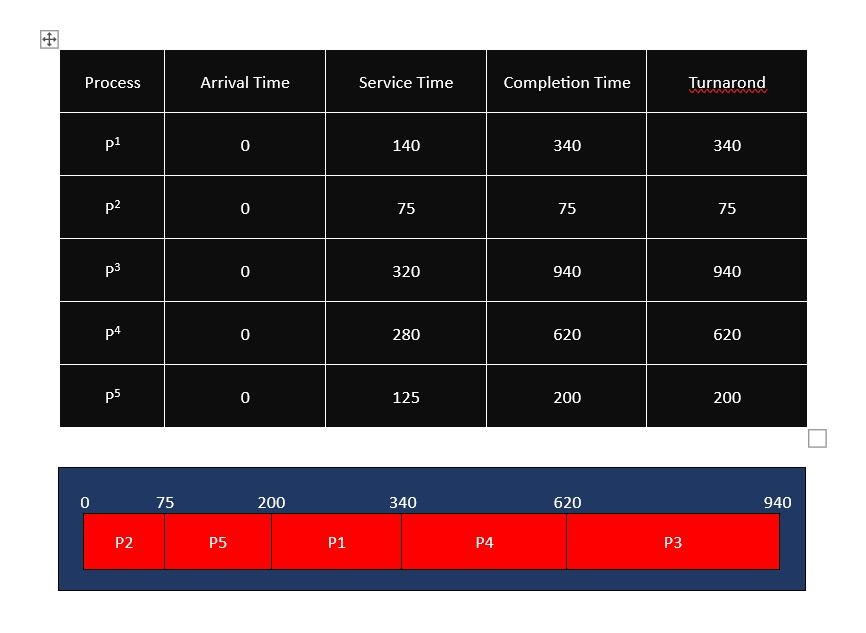
\includegraphics[width=1\textwidth]{asset/sjn-illustration.jpg}
    \caption{Ilustrasi SJN}
    \label{fig:ilustrasi sjn}
\end{figure}

 Dalam Shortest Job Next (SJN), saat memilih pekerjaan berikutnya untuk dijalankan, lihat semua proses dalam status siap dan jalankan yang memiliki waktu layanan tersingkat. Dalam kasus ini, kita perlu mengetahui waktu layanan pada setiap titik waktu tertentu. Ini adalah algoritma non -preemptif.Pekerjaan baru tidak akan diberi kesempatan pada CPU hingga pekerjaan saat ini selesai meskipun pekerjaan baru tersebut lebih pendek.
 \subsubsection{Konsep dan Istilah Utama}
\begin{itemize}
    \item Waktu layanan adalah jumlah waktu yang dibutuhkan suatu proses atau pekerjaan untuk menyelesaikan eksekusi setelah mulai berjalan pada CPU. Waktu layanan juga dikenal sebagai burst time.
    \item Waktu kedatangan adalah waktu saat suatu proses tiba dan siap untuk dieksekusi di CPU atau antrean penjadwalan.
    \item Waktu penyelesaian adalah titik waktu ketika suatu proses menyelesaikan eksekusinya.
    \item Waktu penyelesaian adalah total waktu yang dibutuhkan oleh suatu proses untuk menyelesaikan eksekusinya, sejak proses tersebut tiba di antrian siap hingga proses tersebut menyelesaikan eksekusi. Waktu penyelesaian dihitung sebagai waktu penyelesaian dikurangi waktu kedatangan.
    \item Algoritma penjadwalan nonpreemptif adalah algoritma yang mana proses yang telah mulai dijalankan akan terus berlanjut hingga proses tersebut selesai. Proses baru tidak diperbolehkan mengganggu proses yang sedang berjalan.
\end{itemize}

\subsubsection{Contoh Kasus Shortest Job Next (SJN) Scheduling}
    \begin{itemize}
        \item Pada server, terdapat beberapa proses yang membutuhkan CPU untuk waktu yang berbeda-beda. Misalnya, proses A membutuhkan 5 detik CPU, proses B membutuhkan 3 detik, dan proses C membutuhkan 1 detik.
        \item SJN memilih proses dengan waktu eksekusi tersingkat terlebih dahulu.Dalam kasus ini, sistem akan menjalankan proses C terlebih dahulu,kemudian B, dan terakhir A. Ini mengurangi waktu tunggu rata-rata karena proses yang lebih singkat diselesaikan lebih cepat.
    \end{itemize} 


 
    
\subsection{Process Creation and Termination}
Details how processes are created and terminated by the operating system, including:
\begin{itemize}
    \item Process spawning
    \item Process termination conditions
\end{itemize}

\subsection{Introduction to Threads}
This section introduces the concept of threads and their relation to processes, covering:
\begin{itemize}
    \item Single-threaded vs. multi-threaded processes
    \item Benefits of multithreading
\end{itemize}

\begin{figure}[h]
    \centering
    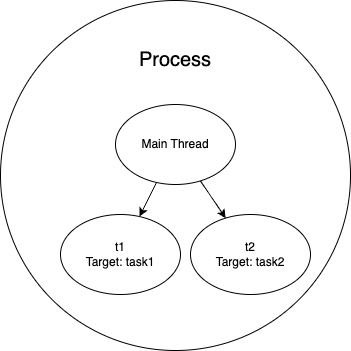
\includegraphics[width=0.5\textwidth]{/Users/khawaritzmi/Unhas/os_report_mid2024/a_class/asset/example.png}  % Sesuaikan nama file dan ukurannya
    \caption{Ini adalah gambar contoh dari multithreading.}
    \label{fig:contoh_gambar}
\end{figure}

Seperti yang terlihat pada Gambar \ref{fig:contoh_gambar}, inilah cara menambahkan gambar dengan keterangan.

\subsection{File Systems}
File systems provide a way for the operating system to store, retrieve, and manage data. This section explains:
\begin{itemize}
    \item File system structure
    \item File access methods
    \item Directory management
\end{itemize}

\subsection{Input and Output Management}
Input and output management is key for handling the interaction between the system and external devices. This section includes:
\begin{itemize}
    \item Device drivers
    \item I/O scheduling
\end{itemize}

\subsection{Deadlock Introduction and Prevention}
Explores the concept of deadlocks and methods for preventing them:
\begin{itemize}
    \item Deadlock conditions
    \item Deadlock prevention techniques
\end{itemize}

\subsection{User Interface Management}
This section discusses the role of the operating system in managing the user interface. Topics covered include:
\begin{itemize}
    \item Graphical User Interface (GUI)
    \item Command-Line Interface (CLI)
    \item Interaction between the user and the operating system
\end{itemize}

\subsection{Virtualization in Operating Systems}
Virtualization allows multiple operating systems to run concurrently on a single physical machine. This section explores:
\begin{itemize}
    \item Concept of virtualization
    \item Hypervisors and their types
    \item Benefits of virtualization in modern computing
\end{itemize}

\section{Assignments and Practical Work}
\subsection{Assignment 1: Process Scheduling}
Students were tasked with implementing various process scheduling algorithms (e.g., FCFS, SJN, and RR) and comparing their performance under different conditions.
\subsubsection{Group 1}
\begin{python}
    class Process:
    def __init__(self, pid, arrival_time, burst_time):
        self.pid = pid
        self.arrival_time = arrival_time
        self.burst_time = burst_time
        self.completion_time = 0
        self.turnaround_time = 0
        self.waiting_time = 0
\end{python}

\begin{table}[htbp] % Optional: For floating position
    \centering
    \begin{tabular}{|c|c|c|} % Defines number of columns and alignment (c = center, l = left, r = right). '|' creates vertical lines.
    \hline
    Header 1 & Header 2 & Header 3 \\ % Column headers
    \hline
    Row 1, Column 1 & Row 1, Column 2 & Row 1, Column 3 \\ % First row of data
    \hline
    Row 2, Column 1 & Row 2, Column 2 & Row 2, Column 3 \\ % Second row of data
    \hline
    \end{tabular}
    \caption{Your table caption} % Optional: For adding a caption
    \label{tab:your_label} % Optional: For cross-referencing the table
\end{table}
\subsection{Assignment 2: Deadlock Handling}

\subsubsection{Pertanyaan dan Jawaban serta Implementasi Kode Python untuk Deadlock Handling}

\textbf{Pertanyaan :} 

\vspace{0.2cm}

Jelaskan bagaimana deadlock dapat terjadi dalam kode di bawah!

\vspace{0.2cm}

\begin{python}
import threading
import time

class SumberDaya:
    def _init_(self, nama):
        self.nama = nama
        self.lock = threading.Lock()

def skenario_deadlock(sumber_a, sumber_b):
    def thread_1():
        # Kunci sumber daya dalam urutan yang sama di kedua thread
        with sumber_a.lock:
            print(f"Thread 1: Mengunci {sumber_a.nama}")
            time.sleep(1)  # Simulasikan kerja
            with sumber_b.lock:
                print(f"Thread 1: Mengunci {sumber_b.nama}")
        print("Thread 1 selesai")

    def thread_2():
        # Kunci sumber daya dalam urutan yang sama di kedua thread
        with sumber_a.lock:
            print(f"Thread 2: Mengunci {sumber_a.nama}")
            time.sleep(1)  # Simulasikan kerja
            with sumber_b.lock:
                print(f"Thread 2: Mengunci {sumber_b.nama}")
        print("Thread 2 selesai")

    t1 = threading.Thread(target=thread_1)
    t2 = threading.Thread(target=thread_2)

    t1.start()
    t2.start()
    
    t1.join()
    t2.join()

# Buat dua sumber daya
sumber_a = SumberDaya("Sumber Daya A")
sumber_b = SumberDaya("Sumber Daya B")
skenario_deadlock(sumber_a, sumber_b)
\end{python} 

\textbf{Jawaban:} Deadlock terjadi ketika dua thread mencoba mengunci dua sumber daya dalam urutan yang berlawanan. Dalam kode ini:

\begin{itemize}
    \item {thread\_1} mengunci {sumber\_a} terlebih dahulu, lalu mencoba mengunci {sumber\_b}.
    \item {thread\_2} mengunci {sumber\_b} terlebih dahulu, lalu mencoba mengunci {sumber\_a}. Jika {thread\_1} mengunci {sumber\_a} dan {thread\_2} mengunci {sumber\_b} pada saat yang sama, kedua thread akan menunggu selamanya untuk sumber daya lain yang tidak pernah tersedia, sehingga terjadi deadlock.
\end{itemize}




\subsection{Assignment 3: Multithreading and Amdahl's Law}
This assignment involved designing a multithreading scenario to solve a computationally intensive problem. Students then applied **Amdahl's Law** to calculate the theoretical speedup of the program as the number of threads increased.

\subsection{Assignment 4: Simple Command-Line Interface (CLI) for User Interface Management}
Students were tasked with creating a simple **CLI** for user interface management. The CLI should support basic commands such as file manipulation (creating, listing, and deleting files), process management, and system status reporting.

\subsection{Assignment 5: File System Access}
In this assignment, students implemented file system access routines, including:
\begin{itemize}
    \item File creation and deletion
    \item Reading from and writing to files
    \item Navigating directories and managing file permissions
\end{itemize}

\section{Conclusion}
The first half of the course introduced core operating system concepts, including process management, scheduling, multithreading, and file system access. These topics provided a foundation for more advanced topics to be covered in the second half of the course.

\end{document}
